SafeStreets is a software that needs to be fast and reliable in order to allow the user to send a report immediately after he detects a violation. The goal is to design an architecture that can offer a good level of performance with respect to scalability and portability. The system is splitted into three separate applications: a mobile front-end application for the users, a Web application for the authorities and a back-end system that manages all the operations. More in details, the user application is a light-weight crossplatform mobile client; with this approach, the client side is relieved from the computation and the result is a fast application for the users. With this mobile application, users can perform the main functions related to them, such as: registration, login, send reports, consult the history of their reports and watch a map with the MDS. The application is connected to the backend service, which is the part of the architecture that handles all the main operations regarding the elaboration of data. In fact, the backend is the core of the architecture: it manages the incoming requests and handles the interaction with the third party system for the plate recognition. This is fundamental because the authorities need to receive the plate number in order to immediately identify the right vehicle. This operation is done by sending the picture taken by the user to an external service that finds the plate number in the image and sends it back to the system as a string. Moreover the backend provides an interface that interacts with the cloud-based database in which the data will be saved. Finally, it provides the functions to compute (on request) the MDS and other useful metrics. As an optional feature the backend can be configured to interact with a municipality service that offers data about car accidents. In this case, the backend compares the information sent with the data stored in the database. Therefore, it tries to identify the potentially unsafe areas and suggests possible interventions.\newline The Web application takes advantage of the interactions with the remote database offered by the backend to provide a simple interface for the authorities in order to let them consult the stored data: they can query all reports, filter them by some specific criterias and analyze the data to get the statistics that they desire. \newline
The following UML diagrams represent the global structure of SafeStreets. In particular, the class diagram pictures the main entities involved in the software functioning and the state diagram is a general representation of one of the main functions of the system.
\begin{figure}[H]
    \centering
    \includegraphics[width=0.8\textwidth]{UML_diagrams/Class}
    \caption{Class diagram}
    \label{fig:class_diagram}
\end{figure}
\begin{figure}[H]
    \centering
    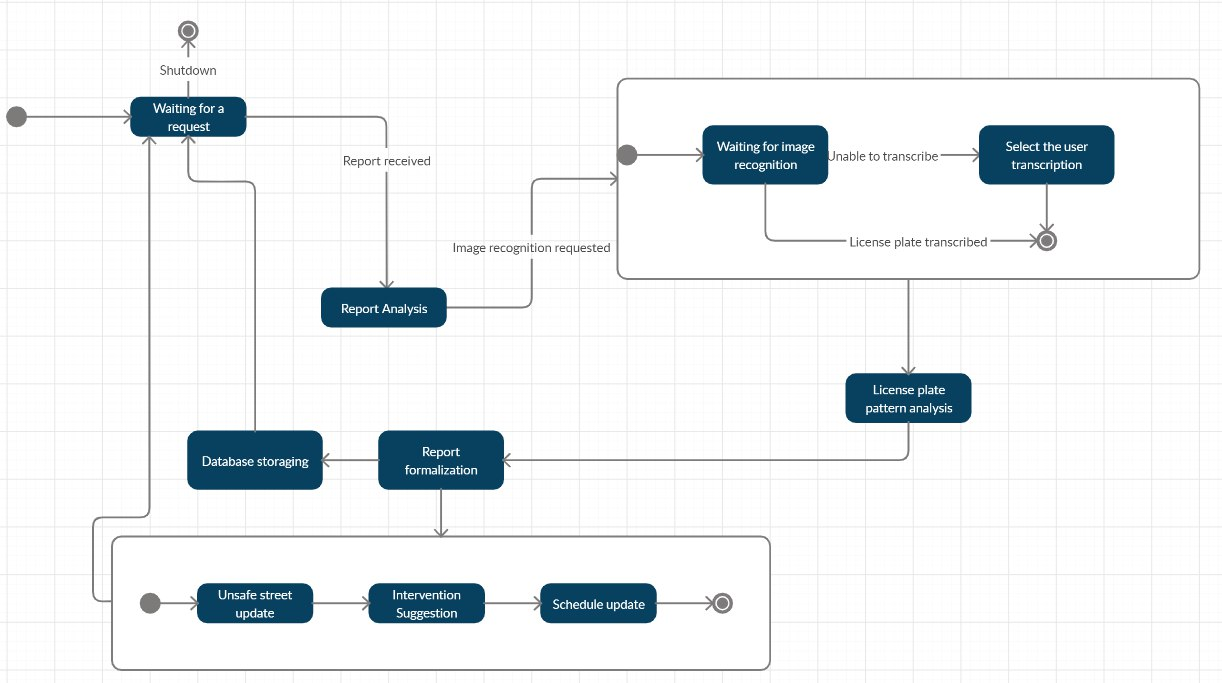
\includegraphics[width=1.0\textwidth]{UML_diagrams/State}
    \caption{Report state diagram}
    \label{fig:state}
\end{figure}
\newpage
